\documentclass{beamer}
\title{Assignment 1: Tools}
%\subtitle{}
\author{$<$Name of Business Manager$>$}
\subject{Tools}
\usetheme{Darmstadt}
\usecolortheme{beaver}
\useoutertheme{infolines}
\useinnertheme{circles}
\usepackage{comment}

\setbeamertemplate{footline} { 
  \leavevmode
  \hbox{\begin{beamercolorbox}[wd=.5\paperwidth, ht=2.5ex, dp=1.125ex,
        leftskip=.3cm, rightskip=.3cm plus1fill]{author in head/foot}
      \usebeamerfont{author in head/foot}\insertshortdate
  \end{beamercolorbox}
  \begin{beamercolorbox}[wd=.5\paperwidth,ht=2.5ex, dp=1.125ex, 
        leftskip=.3cm plus1fill, rightskip=.3cm]{title in head/foot}
    \usebeamerfont{title in head/foot}\insertshortauthor
  \end{beamercolorbox}}
  \vskip0pt
}

\begin{document}
\maketitle
\frame{
  \transdissolve[duration=0.25]
  \frametitle{The Team}
  \framesubtitle{Ryan Alcoran, Joe Lee, Shivalik Narad, Nam Phan, Swapna Vemparala, Amber Wong}
  \begin{center}
    {\Huge Team Q 06}\\[1em]
  \end{center}
  \pause
  \begin{itemize}
    \item Alcoran, Ryan \{unspecified\}
      \pause
    \item Lee, Joe \{Project Manager, Business Manager\}
      \pause
    \item Narad, Shivalik \{unspecified\}
      \pause
    \item Phan, Nam \{Development Manager, Test Manager\}
      \pause
    \item Vemparala, Swapna \{Project Manager, Risk Manager, Business Manager\}
    \pause
    \item Wong, Amber \{unspecified\}
  \end{itemize}
}

%Introduction
\frame{
  \transdissolve[duration=0.25]
  \frametitle{Software Configuration Management (SCM)}
  \framesubtitle{Tracking and controlling changes in software}
  \begin{center}
  	{\Huge Language: Java} \\[1em]
  	\pause
    {\Huge Tools} \\[2em]
    \pause
    \begin{itemize}
      \item Software Configuration Management: {\bf EGit}
        \pause
      \item Software Hosting Facility: {\bf Github}
        \pause
        \item Standalone Bug Tracker: {\bf Codebeamer}
        \pause
        \item Editor and IDE: {\bf Eclipse}
        \pause
        \item  Project Management: {\bf OpenProject}

    \end{itemize}
   
  \end{center}
}

%Egit
\frame{
  \transdissolve[duration=0.25]
  \frametitle{Software Configuration Management (SCM)}
  \framesubtitle{Tracking and controlling changes in software}
  \begin{center}
    {\Huge EGit} \\[1em]
    \pause
    "The EGit project is implementing Eclipse tooling on top of a Java implementation of Git."\\[2em]
    \pause
    \begin{itemize}
      \item free, open source, designed for branching and merging
        \pause
      \item decentralized model (everyone has own copy of repository, which can later be merged)
        \pause
      \item Can be integrated into Eclipse, using a plug-in.
    \end{itemize}
  \end{center}
}

%Egit compare
\frame{
  \transdissolve[duration=0.25]
  \frametitle{Software Configuration Management (SCM)}
  \framesubtitle{Tracking and controlling changes in software}
  \begin{center}
    {\Huge EGit compare to Others} \\[1em]
    \pause
        
    \begin{flushleft}
    {\Large Subversion}
	\end{flushleft}
	\pause
    \begin{itemize}
      \item free, open source, actively developed
        \pause
      \item easier to use than Git (more tools available for non-technical users, error messages are easier to understand)
      \pause
      \item centralized model (everyone has a working copy and changes are submitted to central repository)
      \pause
    \end{itemize}
    
    \begin{flushleft}
    {\Large LibreSource}
	\end{flushleft}
	\pause
    \begin{itemize}
      \item free, open source, maintained and new features under development
       
    \end{itemize}
  \end{center}
}

%Egit install
\frame{
  \transdissolve[duration=0.25]
  \frametitle{Software Configuration Management (SCM)}
  \framesubtitle{Tracking and controlling changes in software}
  \begin{center}
    {\Huge EGit Installation} \\[1em]
    \pause
    \begin{figure}[h!]   
      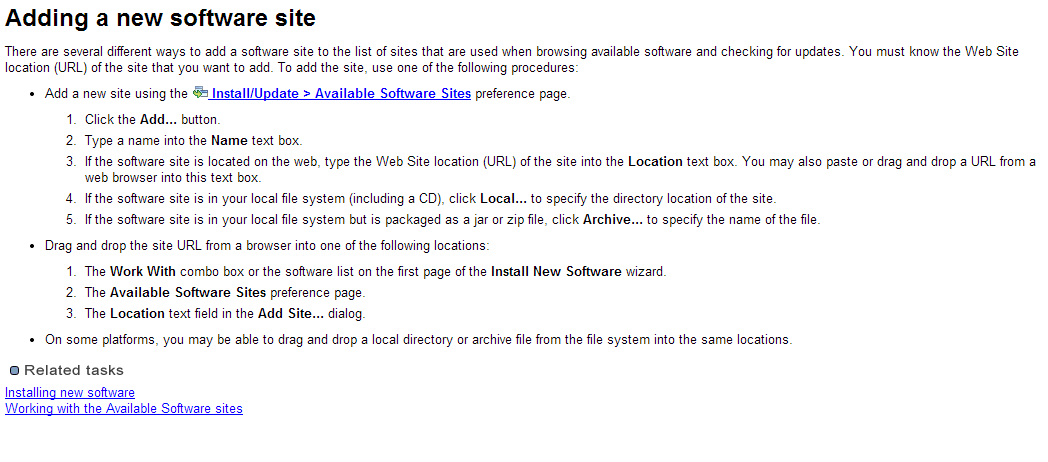
\includegraphics[width=0.8\textwidth]{Screenshots/egit/egit1.PNG}
  \caption{Instruction to install Egit into Eclispe}
\end{figure}
	
  \end{center}
}

\frame{
  \transdissolve[duration=0.25]
  \frametitle{Software Configuration Management (SCM)}
  \framesubtitle{Tracking and controlling changes in software}
  \begin{center}
    {\Huge EGit Installation} \\[1em]
    \begin{figure}[h!]   
      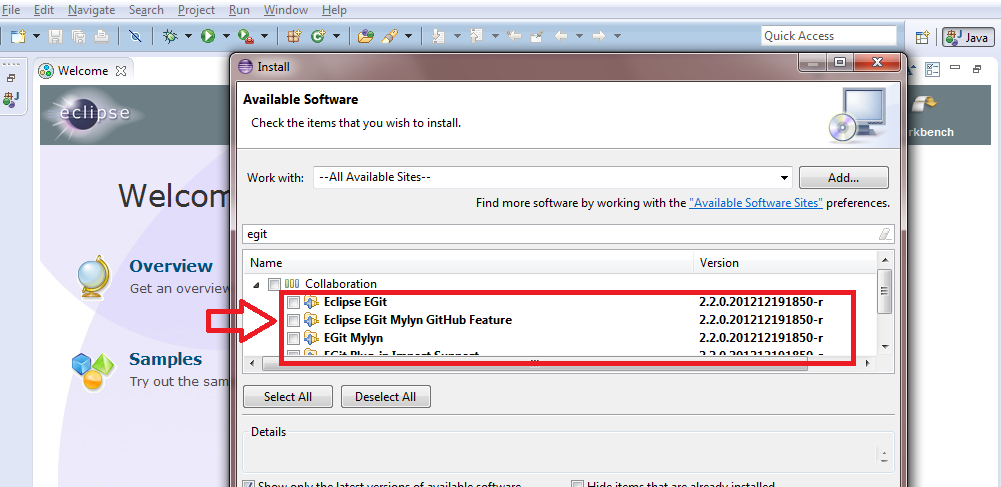
\includegraphics[width=0.8\textwidth]{Screenshots/egit/egit2.PNG}
  \caption{Instruction to install Egit into Eclispe}
\end{figure}
	
  \end{center}
}

%Github
\frame{
  \transdissolve[duration=0.25]
  \frametitle{Software hosting facilities}
  \begin{center}
    {\Huge GitHub} \\[1em]
    \pause
    Public code hosting.
  \end{center}
}

%Codebeamer
\frame{
  \transdissolve[duration=0.25]
  \frametitle{Standalone bug trackers}
  \begin{center}
    {\Huge CodeBeamer} \\[1em]
    \pause
    "CodeBeamer is a web based Collaborative Application Lifecycle Management and Requirements management tool for distributed software development" \\[2em]
   
  \end{center}
  \pause
  \begin{itemize}
    \item Proprietary, free version
      \pause
    
    \item Backend: MySQL, Oracle, Apache Derby or Postgres
    \pause
    \item CodeBeamer is the award winning Collaborative Requirements Management (RM) and Application Lifecycle Management (ALM) solution for distributed software development
  \end{itemize}
}
%Codebeamer compare
\frame{
  \transdissolve[duration=0.25]
  \frametitle{Standalone bug trackers}
  \begin{center}
    {\Huge CodeBeamer compare to Others} \\[1em]
    \pause
       
  \end{center}
   
    {\Large Bugzilla}
	
	\pause
    \begin{itemize}
      \item MPL (free, open source, developed/maintained by Mozilla Foundation)
        \pause
      \item backend: MySQL, Oracle, PostgreSQL, SQLite
      \pause
      
    \end{itemize}
    
    
    {\Large Google Code Hosting}

	\pause
    \begin{itemize}
      \item Proprietary, hosted; available for open source projects (by Google Code)
        \pause
      \item BigTable backend (also proprietary)
    \end{itemize}
}
%IDE	
\frame{
  \transdissolve[duration=0.25]
  \frametitle{Editors and IDEs}
  \pause
  \begin{center}
  \begin{itemize}
    \item {\bf NetBeans IDE}
      \pause
      \begin{itemize}
        \item Dual-licensed under Common Development and Distribution License (CDDL) v1.0 and GNU GPLv2, with some components released other third-party licenses
          \pause
        \item Create and debug rich web and mobile applications using the latest HTML5, \pause JavaScript, \pause and CSS3 standards.
          \pause
        \item Page inspector
          \pause
        \item CSS style editor
          \pause
        \item JavaScript editor
          \pause
        \item JavaScript debugger
          \pause
        \item Support for PHP, Java, C, C++
          \pause
      \end{itemize}
    \item {\bf Eclipse}
      \pause
      \begin{itemize}
        \item License: MPL
          \pause
        \item IDE framework
          \pause
        \item Tools framework\\[1em]
      \end{itemize}
      \pause
  \end{itemize}
  \end{center}
}

\frame{
  \transdissolve[duration=0.25]
  \frametitle{Editors and IDEs}
  \begin{itemize}
    \item {\bf GNU Emacs}
      \pause
      \begin{itemize}
        \item License: GNU GPLv3
          \pause
        \item Text editor
          \pause
        \item Extensible
          \pause
        \item Customizable
      \end{itemize}
  \end{itemize}
}

\frame{
  \transdissolve[duration=0.25]
  \frametitle{Project Management Tools}
  \begin{center}
    {\Huge OpenProj}\\[1em]
    \pause
    Common Public Attribution License (CPAL) 1.0\\[2em]
    \pause
    {\Huge Agilefant \pause (maybe?)}\\[1em]
    \pause
    Expat (MIT) License
  \end{center}
}

\end{document}
